\subsection{Important definitions}

\begin{definition}
    Let $K$ and $L$ be two simplicial complexes, and $V_K, V_L$ their set of 
    vertices. A simplicial map between $K$ and $L$ is a map $f : V_K \to V_L$ such that
    $\forall \sigma \in K, f(\sigma) \in L$. When there is no risk of
    confusion, we may denote a simplicial map $f : K \to L$ instead of $f :
    V_K \to V_L$.
    
    We define a linear map $f_n : C_n(K) \to C_n(L)$ as follows (definition on the simplices, and
    extended by linearity):
    $$
    f_n : \sigma \mapsto f(\sigma) \mathbbm{1}\{dim(f(\sigma)) = n\}
    $$
\end{definition}

\begin{definition}
    By definition of the homology groups, we have defined a map 
    $$(f_n)_* : H_n(K) \to H_n(L).$$ It is called the induced map in homology.
    Explicitly, the map $(f_n)_*$ can be described as follows (the following formula is to be
    read modulo boundaries):
    $$c = \sum_{\sigma \in K_{(n)}} \epsilon_{\sigma} \cdot \sigma \mapsto
    \sum_{\sigma \in K_{(n)}} \epsilon_{\sigma} \cdot f_n(\sigma).$$
\end{definition}

\begin{definition}
    Let $i \ge 0$, $t_0 \ge 0$ and consider a cycle $c \in
    H_i(Cech^{t_0}(X))$. Its death time is
    $$\sup\{t \ge t_0, (i^t_{t_0}) (c) \neq 0\}$$
    and its birth time is
    $$\inf\{t \ge t0, (i^{t_0}_t)^{-1}(\{c\}) \neq \emptyset\}$$

    \begin{center}
        {\it persistence = death time - birth time}
    \end{center}
\end{definition}

\begin{definition}
    A persistence module $\mathbb{V}$ over $\R^+$ with coefficients in
    $\Z/2\Z$ is a pair $(\mathbb{V}, \mathbbm{v})$ where $\mathbb{V} = (V^t)_{t
    \in \R^+}$ is a family of $\Z/2\Z$-vector spaces, and $\mathbbm{v} = (v_s^t
    : V^s \to V^t)_{s \le t \in \R^+}$ a family of linear maps such that:
    \begin{enumerate}
        \item for every $t \in \R^+, v^t_t$ is the identity map,
        \item for every $r,s,t \in \R^+$ such that $r \le s \le t$, we have
        $v_s^t \circ v_r^s = v_r^t$
    \end{enumerate}
When the context is clear, we may denote $\mathbb{V}$ instead of $(\mathbb{V}, \mathbbm{v})$. 
\end{definition}

\begin{definition}
    An isomorphism between two persistence modules $\mathbb{V}$ and
    $\mathbb{W}$ is a family of isomorphisms of vector spaces $\phi = (\phi_t:
    V^t \to W^t)_{t\in \R^+}$ such that the following diagram commutes for
    every $s \le t \in \R^+$.
    
    \begin{figure}[H]
        \begin{center}
            \begin{tikzpicture}
                \node at (0,0) (vs) {$V^s$};
                \node[right =1cm of vs]  (vt){$V^t$};
                \node[below =1cm of vs]  (ws){$W^s$};
                \node[below =1cm of vt]  (wt){$W^t$};
                \draw[->,>=stealth] (vs) --node[above]{$v^t_s$} (vt);
                \draw[->,>=stealth] (vs) --node[left]{$\phi_s$} (ws);
                \draw[->,>=stealth] (vt) --node[right]{$\phi_t$} (wt);
                \draw[->,>=stealth] (ws) --node[below]{$w^t_s$} (wt);
            \end{tikzpicture}            
        \end{center}
    \end{figure} 
\end{definition}

\begin{definition}
    Let $(\mathbb{V}, \mathbbm{v})$ and $(\mathbb{W}, \mathbbm{w})$ be two
    persistence modules. Their sum is the persistence module $V \oplus W$
    defined with the vector spaces $(V \oplus W)^t = V^t \oplus W^t$ and
    the linear maps
    $$(v \oplus w)^t_s : (x,y) \in (V \oplus W)^s \mapsto (v_s^t(x), w_s^t(y))
    \in (V \oplus W)^t.$$
    A persistence module $\mathbb{U}$ is {\it indecomposable} if for every
    pair of persistence modules $\mathbb{V}$ and $\mathbb{W}$ such that
    $\mathbb{U}$ is isomorphic to the sum $\mathbb{V} \oplus \mathbb{W}$, then
    one of the summand has to be a trivial persistence module, that is, equal
    to zero for every $t \in \R^+$. Otherwise, $\mathbb{U}$ is said
    decomposable.
\end{definition}

\begin{definition}
    Let $I \subset \R^+$ be an interval. Intervals have the form $[a, b]$,
    $(a, b]$, $[a, b)$ or $(a, b)$, with $a, b \in \R^+$ such that $a \le b$,
    and potentially $b = +\infty$. The interval module associated to $I$ is
    the persistence module $\mathbb{B}[I]$ with vector spaces
    $\mathbb{B}^t[I]$ and linear maps $v^t_s: \mathbb{B}^s[I] \to
    \mathbb{B}^t[I]$ defined as 
    $$
    \mathbb{B}^t[I] = \begin{cases}
        \Z/2\Z &\text{if } t \in I, \\
        0 &\text{otherwise}
    \end{cases} \text{ and } 
    v_s^t = \begin{cases}
        id &\text{if }s,t \in I \\
        0 &\text{otherwise}
    \end{cases}
    $$
\end{definition}

\begin{definition}
    A persistence module $\mathbb{V}$ decomposes into interval module if there
    exists a set $\{\mathbb{B}_i, i \in I\}$ of interval modules such that
    $\mathbb{V}$ is isomorphic to the sum $\bigoplus_{i \in I} \mathbb{B}_i$;.
    In other words, there exists a multiset $\mathcal{I}$ of intervals of $T$
    such that
    $$\mathbb{V} = \bigoplus_{I\in \mathcal{I}} \mathbb{B}[I].$$
    Multiset means that $\mathcal{I}$ may contain several copies of the same
    interval $I$. 
    Such a module is said decomposable into interval modules, or simply
    decomposable when the context is clear.
\end{definition}

\subsection{Exercises}

\begin{exercise}
    Consider a linear map $f : V \to W$ between vector spaces. Suppose that
    there exists linear subspaces $A \subset V$ and $B \subset W$ such that
    $f(A) \subset B$. Show that one can define a map $f_* : V /A \to W/B $ as
    follows: to any equivalence class $v + A$ of $V /A$, let $f_*(v + A) = f(v) + B$.
\end{exercise}

\begin{proof}
    We have to prove $f_*$ is well-defined. In other words, if $v_1 + A = v_2 + A$, that
    is, $v_1 - v_2 \in A$, then $f(v_1) + B = f(v_2) + B$. In that sense, we must
    prove that $f(v_1) - f(v_2) = f(v_1 - v_2) \in B$. But this is true since by
    hypotheses $v_1 - v_2 \in A \implies f(v_1 - v_2) \in f(A) \subset B$. Then
    $f_*$ is indeed well defined. 

    Let's prove it's linear. Let $\alpha \in \mathbb{F}$, and $v_1, v_2 \in V$. So
    \begin{equation*}
        \begin{split}
            f_*((\alpha v_1 + v_2) + A) &= f(\alpha v_1 + v_2) + B \\
            &= \alpha f(v_1) + f(v_2) + B \\
            &= \alpha(f(v_1) + B) + (f(v_2) + B) \\
            &= \alpha f_*(v_1 + A) + f_*(v_2 + A)
        \end{split}
    \end{equation*}
    The third equation is true because $B = \alpha B + B$, that is, if $b \in B$,
    then $b = \alpha 0 + b \in \alpha B + B$ and in $b \in \alpha B + B$, one can
    find $b_1, b_2 \in B$ such that $b = \alpha b_1 + b_2$. Because of the
    linearity of $B$, we have $b \in B$.  We conclude $f_*$ is a linear map
    induced by $f$ between quotient linear spaces.     
\end{proof}

\noindent\linia

\begin{exercise}
    Let the simplicial $K = \{[0], [1], [2], [3], [4], [5], [0, 1], [1, 2], [2, 3], [3, 4],
    [4, 5], [5, 0]\}$ and  $L = \{[0], [1], [2], [0, 1], [1, 2], [2, 0]\}$.
    Consider the simplicial map $f : i \mapsto i$ modulo 3. Show that the induced map $(f_1)_*$ is zero.
\end{exercise}

\begin{proof}
    We have that $(f_1)_* : H_1(K) \to H_1(L)$, such that $$H_1(K) = \{[0,1] +
    [1,2]+ [2,3] + [3,4] + [4,5] + [5,0], 0\}.$$
    This happens because $Z_1(K)$ has only two elements not equivalents. The
    same can be told about $H_1(L)$. Then 
    \begin{equation*}
        \begin{split}
            (f_1)_*([0,1] + ... + [5,0]) &= f_1([0,1]) + ... + f_1([5,0]) \\
            &= f([0,1]) + ... + f([5,0]) \\
            &= [0,1] + [1,2] + [2,0] + [0,1] + [1,2] + [2,0] = 0
        \end{split}
    \end{equation*}
    And its trivial that $(f_1)_*(0) = 0$ (linear map), what implies the induced map $(f_1)_*$ is zero.
\end{proof}

\noindent\linia

\begin{exercise}
    Fill the empty spaces ( ) in the following proof of Brouwer’s fixed point theorem.
\end{exercise}

\begin{proof}
    Let $f : \bar{\B}(0,1) \to \bar{\B}(0,1)$ be a continuous map, where
    $\bar{\B}(0,1)$ denotes the closed unit ball of $\R^n$. Let us show that
    $f$ admits a fixed point (i.e., an element $x \in \bar{\B}(0, 1)$ such
    that $f(x) = x$). By contradiction, suppose that it is not the case. We
    can build an application $F : \bar{\B}(0,1) \to \sphere(0, 1) \subset  \bar{\B}(0,1)$, such that
    $F$ restricted to $\sphere(0, 1)$ is the identity. To do so, define $F(x)$ as
    the first intersection point between the half-line $[x, f(x))$ and
    $\sphere(0, 1)$. 
    
    Denote the inclusion $i: \sphere(0, 1) \to \B(0, 1)$. We
    have that $F \circ i: \sphere(0, 1) \to \sphere(0, 1)$ is the identity. By
    functoriality of homology, we obtain, for all $i \ge 0$, the commutative
    diagrams. 

    \begin{figure}[H]
        \begin{center}
            \begin{tikzpicture}
                \node at (0,0) (s1) {$\sphere(0,1)$};
                \node[right =1cm of s1]  (b1){$\bar{\B}(0,1)$};
                \node[right =1cm of b1]  (s2){$\sphere(0,1)$};
                \draw[->,>=stealth] (s1) --node[above]{$i$} (b1);
                \draw[->,>=stealth] (b1) --node[above]{$F$} (s2);
                \draw[->,>=stealth] (s1) edge[bend right=30]node[below]{$id$}
                (s2);
                
                \node at (7,0) (hs1) {$H_i(\sphere(0,1))$};
                \node[right =1cm of hs1]  (hb1){$H_i(\bar{\B})(0,1)$};
                \node[right =1cm of hb1]  (hs2){$H_i(\sphere(0,1))$};
                \draw[->,>=stealth] (hs1) --node[above]{$i_*$} (hb1);
                \draw[->,>=stealth] (hb1) --node[above]{$F_*$} (hs2);
                \draw[->,>=stealth] (hs1) edge[bend
                right=30]node[below]{($id_*$)} (hs2);
            \end{tikzpicture}            
        \end{center}
    \end{figure}

But choosing $i = n - 1$, we have $H_i(\sphere(0, 1)) \simeq (\Z/2\Z),
H_i(\bar{\B}(0, 1)) \simeq (0)$ and the following diagram cannot commute:

\begin{figure}[H]
    \begin{center}
        \begin{tikzpicture}
            \node at (0,0) (s1) {($\Z/2\Z$)};
            \node[right =1cm of s1]  (b1){$0$};
            \node[right =1cm of b1]  (s2){($\Z/2\Z$)};
            \draw[->,>=stealth] (s1) -- (b1);
            \draw[->,>=stealth] (b1) -- (s2);
            \draw[->,>=stealth] (s1) edge[bend right=30]node[below]{$id$}
            (s2);
        \end{tikzpicture}            
    \end{center}
\end{figure}

\end{proof}

\noindent\linia

\begin{exercise}
    Show that the interval modules are indecomposable.
\end{exercise}

\begin{proof}
    WLet $\mathbb{V}$ and $\mathbb{W}$ two persistence modules whose sum is isomorphic to $\mathbb{B}[I]$. Then there is $\phi = (\phi^t)_{t \in
    \R^+}$ such that $\mathbb{B}^t[I] \overset{\phi^t}{\to} (V \oplus W)^t$ are
    isomorphic. If $t \not \in I$, We have that $\mathbb{B}^t[I] = 0$ is
    isomorphic to  $(V \oplus W)^t$, what implies $(V \oplus W)^t = (0,0)$ and
    we are done. Otherwise, if $t \in I$, we have $(V \oplus W)^t$ and
    $\Z/2\Z$ are isomorphic. It's clear that $dim(\Z/2\Z) = 1$, because the
    bases only need one element. We claim that $dim((V \oplus W)^t) = 1$. We
    already know $\{\phi^t(1 + \Z)\}$ is a set of independent sets of $(V
    \oplus W)^t$ and we shall prove it spans the space. Take $(v,w) \in (V
    \oplus W)^t$. Then, for some $e \in \Z/2\Z$,
    $$
    (v,w) = \phi^t(e) = \phi^t((1 + \Z)\alpha) = \alpha \phi^t(1 + \Z).
    $$
    Therefore $1 = dim((V + W)^t) = dim(V^t) + dim(W^t) \implies dim(V^t) = 0$
    xor $dim(W^t) = 0$, that is, $V^t = 0$ xor $W^t = 0$. In special we have for
    all $t$, we have $V^t = 0$ or $W^t = 0$.  Suppose $V^t \neq 0$ and $W^s
    \neq 0$, for some $t,s \in \R^+$. We already proved that if $t \not \in
    I$, then $V^t = 0$ and if $s \not \in I$, then $W^s = 0$, so we don't need
    to consider these cases. 

    We know $W^t = 0$ and $V^s = 0$ by what we've proved in the first
    paragraph. By the commutative property and supposing $s \le t$ with no
    loss of generality, 

    \begin{figure}[H]
        \begin{center}
            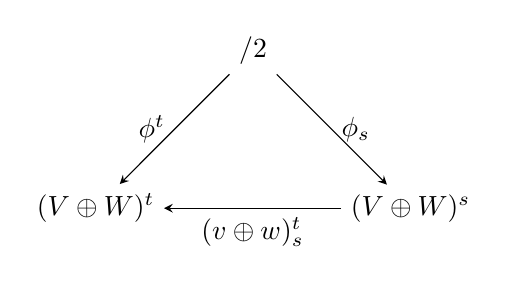
\begin{tikzpicture}
                \node at (0,0) (z) {$\Z/2\Z$};
                \node at (-2,-2)  (vwt){$(V \oplus W)^t$};
                \node at (2,-2)  (vws){$(V \oplus W)^s$};

                \draw[->,>=stealth] (z) --node[left]{$\phi^t$} (vwt);
                \draw[->,>=stealth] (z) --node[right]{$\phi_s$} (vws);
                \draw[->,>=stealth] (vws) --node[below]{$(v \oplus w)_s^t$} (vwt);
            \end{tikzpicture}            
        \end{center}
    \end{figure} 
    Therefore,
    $$
    \phi^t(1 + \Z) = (v,0) \text{ and } \phi^s(1 + \Z) = (0,w), \text{ then } v_s^t(0) = v, w_s^t(w) = 0 
    $$
    Alternatively 
    $$
    \phi^t(0 + \Z) = (0,0) \text{ and } \phi^s(0 + \Z) = (0, 0), \text{ then } v_s^t(0) = 0 
    $$
    This is clearly a contradiction. 
\end{proof}

\noindent\linia

\begin{exercise}
    Let $\mathcal{M}$ be the unit circle of $\R^2$, and $X \subset \R^2$ a
    finite subset. Denote the Hausdorff distance $\epsilon =
    d_H(X,\mathcal{M})$. Suppose that $\epsilon$ is small enough. Let
    $\mathbb{U}$ denote the persistence module of the 1st homology of the Cech
    filtration of $X$. Using Theorem 7.3, shows that there exists an interval
    $I$ on which $\mathbb{U}$ is constant and equal to $\Z/2\Z$. Deduce the existence of a bar in the barcode, and give a lower bound on its persistence. Do the
    same with Theorem 7.4.
\end{exercise}

\begin{proof}
    Let's denote $\mathbb{U} = (H_1(Cech^t(X)))_{t \in \R^+}$. 
    By theorem 7.3, 
    if we take $$t \in [4d_H(X,\mathcal{M}),reach(\mathcal{M}) -
    3d_H(X,\mathcal{M}))$$ we have $X^t \approx \mathcal{M}$. Then, by
    Proposition 5.14, we have isomorphic homology groups $H_1(X)$ and
    $H_1(\mathcal{M})$. We know $H_1(circle) = \Z/2\Z$. Then we take $I = [4d_H(X,\mathcal{M}),reach(\mathcal{M}) -
    3d_H(X,\mathcal{M}))$.

    To use Theorem 7.4, we need the additional supposition that $X \subset
    \mathcal{M}$ is finite. If we take  $I=[2d_H(X,\mathcal{M}),
    \sqrt{\frac{3}{5}}reach(\mathcal{M}))$, we have the result.
\end{proof}

\noindent\linia

\begin{exercise}
    Compute the barcode of the filtration of Subsection 6.1: 
    
    \begin{figure}[H]
        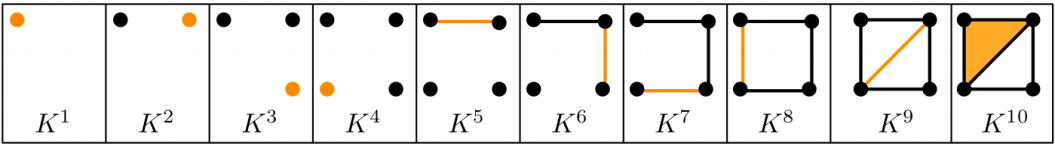
\includegraphics[width=\textwidth]{../images/exercise-52.png}        
    \end{figure}
    \noindent with the
    following filtration values: $t(\sigma) = 0$ for the vertices, $t(\sigma)
    = \frac{1}{2}$ for the edges of the square, and $t(\sigma) =
    \frac{\sqrt{2}}{2}$ for the diagonal edge and the triangle.
\end{exercise}

First let's build the boundary matrix. 

\begin{center}
    \begin{tabular}{|c|c|c|c|c|c|c|c|}
        \hline
        -             & $\sigma_{1,2,3,4}$ & $\sigma_5$ & $\sigma_6$ & $\sigma_7$ & $\sigma_8$ & $\sigma_9$ & $\sigma_{10}$ \\ \hline
        $\sigma_1$    & 0                  & 1          & 0          & 0          & 1          & 0          & 0             \\ \hline
        $\sigma_2$    & 0                  & 1          & 1          & 0          & 0          & 1          & 0             \\ \hline
        $\sigma_3$    & 0                  & 0          & 1          & 1          & 0          & 0          & 0             \\ \hline
        $\sigma_4$    & 0                  & 0          & 0          & 1          & 1          & 1          & 0             \\ \hline
        $\sigma_5$    & 0                  & 0          & 0          & 0          &    0        & 0          & 1             \\ \hline
        $\sigma_6$    & 0                  & 0          & 0          & 0          & 0          & 0          & 0             \\ \hline
        $\sigma_7$    & 0                  & 0          & 0          & 0          & 0          & 0          & 0             \\ \hline
        $\sigma_8$    & 0                  & 0          & 0          & 0          & 0          & 0          & 1             \\ \hline
        $\sigma_9$    & 0                  & 0          & 0          & 0          & 0          & 0          & 1             \\ \hline
        $\sigma_{10}$ & 0                  & 0          & 0          & 0          & 0          & 0          & 0             \\ \hline
    \end{tabular}    
\end{center}

as already placed in the notes. After apply Gauss reduction we obtain 

\begin{center}
    \begin{tabular}{|c|c|c|c|c|c|c|c|}
        \hline
        -             & $\sigma_{1,2,3,4}$ & $\sigma_5$ & $\sigma_6$ & $\sigma_7$ & $\sigma_8$ & $\sigma_9$ & $\sigma_{10}$ \\ \hline
        $\sigma_1$    & 0                  & 1          & 0          & 0          & 0          & 0          & 0             \\ \hline
        $\sigma_2$    & 0                  & 1          & 1          & 0          & 0          & 0          & 0             \\ \hline
        $\sigma_3$    & 0                  & 0          & 1          & 1          & 0          & 0          & 0             \\ \hline
        $\sigma_4$    & 0                  & 0          & 0          & 1          & 0          & 0          & 0             \\ \hline
        $\sigma_5$    & 0                  & 0          & 0          & 0          & 0          & 0          & 1             \\ \hline
        $\sigma_6$    & 0                  & 0          & 0          & 0          & 0          & 0          & 0             \\ \hline
        $\sigma_7$    & 0                  & 0          & 0          & 0          & 0          & 0          & 0             \\ \hline
        $\sigma_8$    & 0                  & 0          & 0          & 0          & 0          & 0          & 1             \\ \hline
        $\sigma_9$    & 0                  & 0          & 0          & 0          & 0          & 0          & 1             \\ \hline
        $\sigma_{10}$ & 0                  & 0          & 0          & 0          & 0          & 0          & 0             \\ \hline
        \end{tabular}
\end{center}

Consider the pairs $(\sigma^{\delta(j)}, \sigma^j)$. We do not have $\delta(j)
= 1$, then $(+\infty, \sigma^1)$ is pair. Since $\delta(5) = 2$, $(\sigma^2,
\sigma^5)$ is another pair. Continuing this reasoning we obtain the pairs 
$$(\sigma^3, \sigma^6), (\sigma^4, \sigma^7), (\sigma^8, + \infty), (\sigma^9,
\sigma^{10}).$$  

We conclude the barcodes will be 

$$\mathcal{I} = \{(0, 1/2), (0, 1/2), (0, 1/2)\}$$